\pdfoutput=1
\documentclass[11pt,a4paper]{article}
\pdfinfoomitdate=1
\pdftrailerid{}
\pdfsuppressptexinfo=-1
\usepackage[T1]{fontenc}
\usepackage[utf8]{inputenc}
\usepackage{mathptmx}
\usepackage[margin=1in]{geometry}
\usepackage{microtype}
\usepackage{amsmath}
\usepackage{graphicx}
\usepackage{booktabs}
\usepackage{array}
\usepackage{tabularx}
\usepackage[font=small,labelfont=bf]{caption}
\usepackage[round,authoryear]{natbib}
\usepackage[hidelinks,pdftitle={Counting by dilution and a width stored at the newline: a partial account of line-breaking in Pythia-410M},pdfauthor={Richard Jeevash},pdfcreator={},pdfproducer={}]{hyperref}
\usepackage{xcolor}
\usepackage{float}
\usepackage{xurl}
\usepackage{placeins}
\renewcommand{\bibfont}{\raggedright}
\usepackage{tikz}
\usetikzlibrary{positioning,arrows.meta,fit}

\setlength{\tabcolsep}{4pt}
\renewcommand{\topfraction}{0.9}\renewcommand{\bottomfraction}{0.6}\renewcommand{\textfraction}{0.1}
\renewcommand{\floatpagefraction}{0.75}\setcounter{topnumber}{3}\setcounter{totalnumber}{4}
% primitive \input, so a row file can end before \bottomrule inside a tabular
\makeatletter\newcommand{\inputrows}[1]{\@@input #1 }\makeatother
\newcolumntype{L}{>{\raggedright\arraybackslash}X}
\newcolumntype{P}[1]{>{\raggedright\arraybackslash}p{#1}}

\title{Counting by dilution and a width stored at the newline:\\a partial account of line-breaking in Pythia-410M}
\author{Richard Jeevash\\
Independent researcher\\
\texttt{jeevash@richardjeevash.com}\\
ORCID \href{https://orcid.org/0009-0005-7812-0939}{0009-0005-7812-0939}}
\date{}

\begin{document}
\maketitle

\begin{abstract}
When text is wrapped at a fixed width, a model that predicts the line breaks must count the characters on the current line, infer the width from earlier lines and compare the two. We give a causal account of parts of this computation in Pythia-410M, proposed in an exploration and then tested in five rounds of frozen predictions on held-out text, including Wikipedia articles written after the model was trained. A head in layer 5 counts characters by how much attention it gives to the line start; a second head removes the per-token bias that this creates; and at the newline the same counting heads store the length of the finished line, which three later heads read at the decision. These two width roles were confirmed at width 60; in eight further conditions of width and text type, the readers held in five and the stored length was detectable in one. The decision is assembled across layers 6 to 18 and damped by two neurons, in MLPs 21 and 23, that suppress the newline. The correction is incomplete on short lines: a token weight of 0.16 remains at width 20. The account is not a complete circuit: with 24 further components it keeps 0.79 of the intact model's variation under mean ablation but only 0.22 under resample ablation. Seven other open models have heads in the same four roles, arranged differently across model families.
\end{abstract}

\section{Introduction}

Much of the text a language model reads is wrapped at a fixed width: source code, plain-text email, poetry, legal documents and old web pages. To predict where such a line ends, a model has to know how many characters the current line already holds, although its input arrives as tokens of varying length; it has to infer the width from the lines it has seen; and it has to compare the two before every word. The task is simple to state, its correct answer is known exactly, and it needs an internal quantity that the input does not supply directly. That makes it a good place to find out how a small model computes something.

The only causal account comes from Claude~3.5 Haiku \citep{gurnee2026manifolds}. There, the character count is represented on curved low-dimensional manifolds, and several attention heads compare it with the line width, each at its own offset from the edge. For open models the evidence is correlational. \citet{sinii2026counting} found the character position linearly decodable in several model families and reported large differences in newline accuracy between them, with GPT-2 far behind Pythia; they call their probe analysis correlational rather than causal. Nobody has shown which components of an open model carry the count, how the width enters, or where the two are compared.

We studied Pythia-410M \citep{biderman2023pythia}. An exploration, run under a charter frozen before it began, proposed an account; we then tested its predictions on text no exploration script had read, with hypotheses, thresholds and analysis frozen, with file digests, before the text was opened. The held-out text was the validation and test splits of WikiText-2 \citep{merity2017pointer}, English Wikipedia articles created between January 2025 and September 2026, which the model cannot have seen in training, Python code and German text. Because the predictions were written after the exploration, these tests show that the account repeats on new text, not that it predicted effects nobody had seen. Appendix~\ref{app:rounds} gives the order in which the tests were run and every frozen result.

The account has four roles and a distributed decision step (Figure~\ref{fig:schematic}).
\begin{itemize}
\item \emph{Counters.} Head L5H6 counts characters by dilution: its attention to the line-start newline falls as the line fills. With L2H7, L4H15 and L5H7 it writes the count into the decision token's state at layer 5 (Section~\ref{sec:count}).
\item \emph{Token correctors.} Because dilution counts tokens as much as characters, the raw count is biased upwards for lines made of many short tokens. Head L5H7, with L4H14 as a weaker second, removes most of that bias, but not all of it on short lines (Section~\ref{sec:count}).
\item \emph{A stored width.} At the line-start newline, the same counting heads record the length of the line that has just ended. This is the model's estimate of the width (Section~\ref{sec:width}).
\item \emph{Readers.} At the decision token, heads L6H2, L8H15 and L17H1 bring the stored length to the decision. L8H15 copies it through the newline's value; L17H1 compares through the newline's key (Section~\ref{sec:width}).
\item \emph{The decision step.} There is no single comparison site. The width is written onto the count's own direction over layers 6 to 14; L17H1 and MLPs 14, 16 and 18 write the result to the newline logit, and two neurons in MLPs 21 and 23 hold it back, suppressing the newline as a break becomes likely. The named parts of this step therefore span layers 6 to 23 (Section~\ref{sec:decision}).
\end{itemize}

The account is partial in two ways that we state up front. First, the token correction is incomplete: at width 40 the intact model gives the number of tokens on the line a small positive weight, a failure of our prediction in every round that tested it, and the leftover weight grows on shorter lines. Second, the named components do not make a complete circuit (Section~\ref{sec:complete}). Kept alone, they reproduce the ranking of breaks and continuations but not the size of the decision. A greedy search added 24 components that bring the circuit's fidelity to 0.785 under mean ablation, but under resample ablation the same circuit reproduces only about a fifth of the decision's variation. The roles are what we can name and test; the rest of the decision is spread over components whose computation we do not explain.

We also asked what is missing in GPT-2 Small \citep{radford2019language}, which does the task poorly: it carries a decodable character count but uses it a quarter as strongly, has no strong dilution counter, and loses the stored width within a few layers. In seven other open models, Pythia-1B, Qwen2.5-0.5B \citep{qwen2024qwen25}, OLMo-2-1B \citep{olmo2024olmo2}, two sizes of Qwen3 \citep{qwen2025qwen3}, Gemma-4-E2B \citep{gemma2026gemma4} and SmolLM2-1.7B \citep{benallal2025smollm2}, frozen cross-model protocols found heads in all four roles: all 29 frozen role tests passed. The heads and their arrangement differ between model families, so there is no single shared circuit, but in two sizes of Qwen3 the same heads, by layer and index, play the same roles (Section~\ref{sec:models}). In an exploratory look at training checkpoints, the counter and the stored width appear first, within the first 1,000 steps, and the corrector, the readers and the late MLPs grow later (Section~\ref{sec:training}).

\begin{figure}[t]
\centering
\resizebox{\textwidth}{!}{%
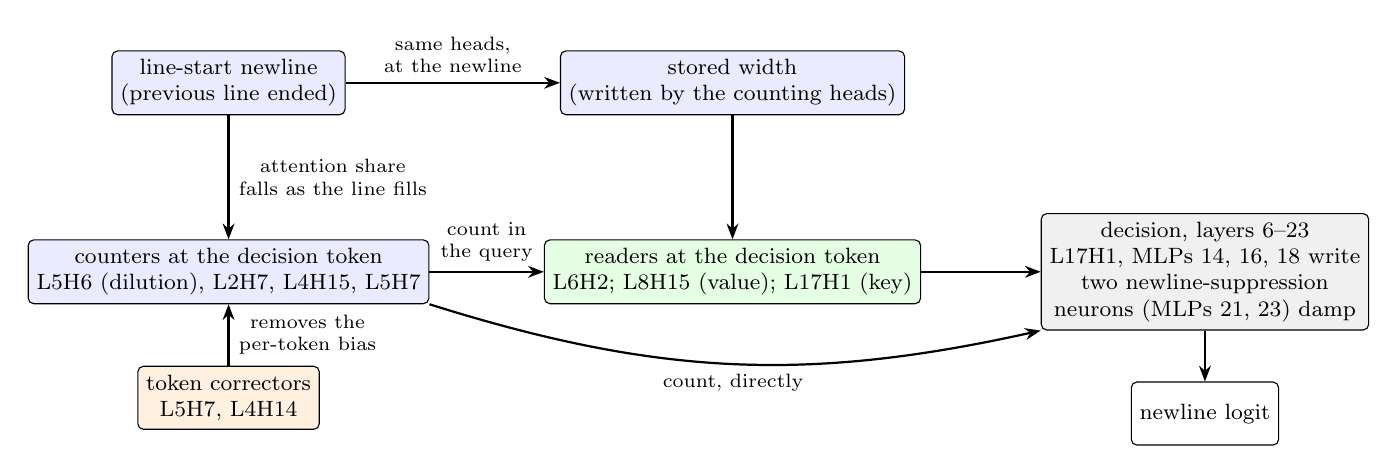
\begin{tikzpicture}[
  box/.style={draw, rounded corners=2pt, align=center, font=\footnotesize, inner sep=3pt, minimum height=0.8cm},
  arr/.style={-{Stealth[length=2mm]}, thick},
  lab/.style={font=\scriptsize, align=center}]
\node[box, fill=blue!8] (nl) at (0,2.4) {line-start newline\\(previous line ended)};
\node[box, fill=blue!8] (cnt) at (0,0) {counters at the decision token\\L5H6 (dilution), L2H7, L4H15, L5H7};
\node[box, fill=orange!12] (cor) at (0,-1.6) {token correctors\\L5H7, L4H14};
\node[box, fill=blue!8] (store) at (6.4,2.4) {stored width\\(written by the counting heads)};
\node[box, fill=green!10] (read) at (6.4,0) {readers at the decision token\\L6H2; L8H15 (value); L17H1 (key)};
\node[box, fill=gray!12] (dec) at (12.4,0) {decision, layers 6--23\\L17H1, MLPs 14, 16, 18 write\\two newline-suppression\\neurons (MLPs 21, 23) damp};
\node[box] (out) at (12.4,-1.8) {newline logit};
\draw[arr] (nl) -- node[lab, right] {attention share\\falls as the line fills} (cnt);
\draw[arr] (cor) -- node[lab, right] {removes the\\per-token bias} (cnt);
\draw[arr] (nl) -- node[lab, above] {same heads,\\at the newline} (store);
\draw[arr] (store) -- (read);
\draw[arr] (cnt) -- node[lab, above] {count in\\the query} (read);
\draw[arr] (read) -- (dec);
\draw[arr] (cnt.south east) to[bend right=15] node[lab, below] {count, directly} (dec.south west);
\draw[arr] (dec) -- (out);
\end{tikzpicture}}
\caption{The account of line-breaking in Pythia-410M tested in this paper. Heads are named by layer and index (L5H6 is head 6 of layer 5). The same four counting heads count at word ends and record the finished line's length at the newline. The figure shows the named parts only; Section~\ref{sec:complete} shows that they are not a complete circuit.}
\label{fig:schematic}
\end{figure}

\section{Related work}

\paragraph{Line-breaking and counting in language models.}
\citet{gurnee2026manifolds} traced line-breaking in Claude~3.5 Haiku. Character counts there lie on curved manifolds, attention heads compare the count with the line width at several offsets, and the distance to the edge and the next word's length are combined into a roughly linear decision. \citet{sinii2026counting} looked for the same structure in open models with probes, principal components and sparse autoencoder features. They found the character position decodable in GPT-2, Pythia, Gemma, Qwen and Llama, a helix-like geometry in several of them, and newline accuracy ranging from poor in GPT-2 to good in Pythia-410M and larger models. The same compare-a-position-with-a-goal motif has since been described in a much larger model \citep{dunefsky2026countdown}. We give a causal account of parts of the computation in a small open model, and compare it with the Haiku account on geometry and on the boundary heads.

\paragraph{Finding and testing circuits.}
Our tools are activation patching and ablation \citep{meng2022locating,wang2023interpretability}, following the practice discussed by \citet{zhang2024patching} and \citet{heimersheim2024patching}. Where we replace components with their mean, we also report resample ablation, which replaces them with values from other inputs, in the spirit of causal scrubbing \citep{chan2022causal}; the two can give different answers, and faithfulness measures are known to depend on such choices \citep{miller2024faithfulness}. Automated circuit discovery \citep{conmy2023automated} searches over edges for a metric; we instead chose components by targeted interventions and tested named sets against random sets of the same size. Earlier circuit studies in small models found heads with positional roles, such as previous-token and induction heads \citep{elhage2021framework,olsson2022induction}, and mechanisms for numerical comparison \citep{hanna2023greaterthan}. In late layers, \citet{stolfo2024confidence} described neurons that regulate a model's confidence: entropy neurons, which act through the final normalisation and write little to the logits directly, and token-frequency neurons. We test whether the late damping of the newline is of this kind.

\section{Task, measures and design}
\label{sec:design}

\paragraph{Text and decision points.}
We used paragraphs of plain prose of 600 to 1,800 characters, joined each paragraph's words with single spaces and wrapped it greedily at a fixed width: each line takes as many whole words as fit. Lines were separated by a single newline. A \emph{decision point} is a token that ends a word, from the third line onwards, where the next true token is either the newline (a break) or a word beginning with a space (a continuation). At each decision point we read the model's log-odds of the newline token. Widths were 40, 60 and 80 characters for most tests; the tests of other widths added widths 20, 30, 100 and 120, and two other kinds of text.

\paragraph{Measures.}
\emph{Separation} is the mean newline log-odds at breaks minus that at continuations with at most 12 characters left; AUROC compares breaks with all continuations. The \emph{token coefficient} is the weight on the number of tokens in the current line, in a regression of the newline log-odds on a linear spline in the characters remaining (knots at 2, 5, 8, 12, 16, 24 and 32) plus that token count, over points with at most 30 characters left. A model that counts characters, not tokens, has a token coefficient near zero. \emph{Width items} pair a prompt that stops at a word end 4 to 14 characters from the edge with the same prompt in which the previous line has been shortened by at least 10 characters; the \emph{width effect} is the resulting change in the log-probability of the newline. We measure it in two ways. The \emph{whole-prompt} width effect compares the two prompts as they stand; it is used wherever components are ablated in both prompts (the stored-width tests H4, the sufficiency tests, the comparison with GPT-2, the training checkpoints, and the stored-length tests in other models). The \emph{patched} width effect leaves the prompt unchanged and replaces only the state of the line-start newline after layer 5 with its state in the shortened prompt, so it measures what the newline token itself stores; it is used for the readers, the decision step and the damping (tests H2, H5, D and M). The reader tests in other models use the same patch, after a layer fixed in each model's protocol, and call it the stored length's effect. When a circuit is kept and the rest ablated, its \emph{fidelity} is one minus the squared error of its newline log-odds against the intact model's, summed over all decision points, relative to the intact log-odds' variance: 1 for a perfect copy, 0 for a constant at the intact mean.

\paragraph{Interventions.}
We used mean ablation (a component's output replaced by its mean over positions in other text), either at every position, at newline tokens only, or at the decision token only; resample ablation (replaced by its value at a point in another paragraph); freezing (a component's output at the decision token held at its value in an unedited run, so that an edit elsewhere can act only through other paths); key-only and value-only patching of a head at the newline; and shifts of the count, in which the class-mean difference for six more characters used is added to the decision token's residual after layer 5. Head outputs are taken before the attention output projection. Every named set was compared with random sets of the same size, drawn from the same layers.

\paragraph{Design.}
The exploration used only the WikiText-2 train split and constructed inputs. Each test on held-out text then had its own protocol: the hypotheses, each with a result that would count against it; the material; the sample rules; the thresholds; and the analysis. The protocol and its scripts were digested and frozen before the text was read. Thresholds were set at about half the explored sizes, or as sign and rank tests, so that the tests guard against an effect vanishing rather than being somewhat smaller. Intervals are 95\% bootstrap intervals over paragraphs or items (2,000 resamples). Each script ran once, and every result is reported. Test labels such as H1b or S4 name the frozen predictions, which are listed with their thresholds in Appendix~\ref{app:rounds}. We label results \emph{exploratory} (from the exploration), \emph{confirmatory} (a frozen prediction tested once on held-out text) or \emph{post hoc} (computed afterwards from saved outputs, changing no verdict).

\section{Behaviour}

Pythia-410M breaks lines well at moderate widths (Table~\ref{tab:behaviour} in Appendix~\ref{app:explore}). At width 60 the newline is its top prediction at 88\% of due breaks, and AUROC is 0.982. GPT-2 Small manages 38\% at the same width, with AUROC 0.851, and gets worse as lines lengthen. Pythia-1B is no better than Pythia-410M. Near the edge, the model's newline logit is explained by the characters remaining ($R^2$ 0.79 at width 60) and hardly at all by the number of tokens in the line ($R^2$ 0.24); adding the token count to the characters adds nothing. Pythia-410M therefore counts characters, and its probabilities are close to calibrated against the true break rate (exploration, Appendix~\ref{app:explore}).

\section{Counting and token correction}
\label{sec:count}

\paragraph{Where the count is written.}
In exploration, shifting the count at the decision token by the class-mean difference for six more characters moved the decision as predicted from layer 5 onwards, and not before, although the count is linearly decodable after layer 4. The count is therefore written at the decision token by layer 5. Ablating every head and MLP in turn identified a small set of heads in layers 2 to 6 on which the decision depends. Among them, L5H6 puts most of its attention on the line-start newline, less as the line fills: a count by dilution. Editing its attention score to the newline moved the decision in a graded way, while a control head's did not.

\paragraph{The per-token bias and its correction.}
A dilution count is also a token count, because every token takes a share of attention. In exploration, re-spelling earlier words with the same number of characters in more tokens showed that, by layer 4, the decision token's state over-counts by a fixed amount per extra token, and that L5H7 removes this dependence. On held-out text, ablating L5H7 gives each token on the line a weight of 0.47 to 0.62 units of log-odds at widths 40, 60 and 80 in rounds 1 to 3 (H1b), while three other heads of the same layer change nothing (H1c). The weight is not the same everywhere: in round 5 it was 0.45 to 0.66 in English at widths 20 to 80, and 0.23 to 0.40 at widths 100 and 120, in code and in German (Table~\ref{tab:tokbias} in Appendix~\ref{app:details}). L4H14 is a second, weaker corrector: ablating it raises the token weight by 0.11 to 0.23 (H3). Exploration had first expected L4H14 to be a source of the bias; that expectation failed there, and H3 then predicted a corrector.

\paragraph{The correction is incomplete on short lines.}
The behavioural half of the prediction failed. H1a required the intact model's token weight to lie within $\pm$0.10 at all three widths. At widths 60 and 80 it did, in all three rounds that tested it. At width 40 the upper bound crossed the limit each time: 0.074 [0.035, 0.113] on the validation split, 0.057 [0.014, 0.103] on the test split and 0.087 [0.046, 0.128] on new text. After two failures the residual itself was predicted for the third test (lower bound above zero) and held. On the new text the width-60 interval also lay above zero, which was not predicted. Between a tenth and a seventh of the weight seen without L5H7 remains.

Counting by dilution explains where this remainder comes from. Each token takes a share of L5H6's attention, and that share falls fastest while the line holds few tokens, so the per-token bias should be largest on short lines, and it is. Without L5H7 the token weight is 0.60 at width 20, 0.28 at width 100 and 0.23 at width 120; the frozen test T3 was the difference between widths 20 and 100 (0.32). Holding the characters used fixed, L5H6's attention to the line start falls by 0.015 per extra token at width 20 and by 0.004 at width 80 (T4). L5H7 removes most of the bias in every condition, code and German included (T5), but less of it on the shortest lines: 73\% at width 20, 85\% at width 30, and 91\% or more at widths of 40 and above. What is left falls as the number of tokens on the line rises (rank correlation $-$0.91 over eleven conditions of width and text; T2): 0.16 at width 20, 0.10 at width 30, 0.05 at width 40, and within 0.04 of zero at widths of 60 to 120 (T1; Figure~\ref{fig:round5}a and Table~\ref{tab:tokbias} in Appendix~\ref{app:details}). German has fewer characters per token than English, so its lines hold more tokens at a given width, and it keeps less of the bias. Code does not follow: it keeps slightly more than English at the same widths (0.061 and 0.036 against 0.050 and 0.015), although its bias without L5H7 is about half as large and L5H7 removes a smaller share of it (80\% and 87\%). The width-40 failure is therefore the visible end of a bias that dilution counting creates on lines of few tokens. At width 120, L5H6's attention again falls steeply per token, which the account does not predict.

\paragraph{Other widths and other text.}
In round 5, Pythia-410M breaks lines at every width from 20 to 120 characters, in code and in German (AUROC 0.871 to 0.986 on held-out text; G1). The counting roles hold throughout: in all eight held-out conditions the four counting heads carry most of a count change, and ablating L5H7 lets the token count in (G2; Table~\ref{tab:general} in Appendix~\ref{app:details}), although at width 20 the count test rests on a single item.

\begin{figure}[t]
\centering
\includegraphics[width=\textwidth]{figures/fig-round5.pdf}
\caption{The token bias, the damping and the fuller circuit on held-out text. (a) The token weight left in the intact model against the mean number of tokens on the line at decision points, for English at seven widths (labelled) and code and German at widths 40 and 60, with 95\% intervals. (b) Change in the log-probability of the likely next token when MLP23.736 and MLP21.1410 are mean-ablated throughout natural text, by that token's intact probability. (c) Fidelity of the round-4 circuit plus the first components of the fidelity path, under mean and under resample ablation; the shaded bars at 24 show, for each ablation, the range of five random sets of the same composition.}
\label{fig:round5}
\end{figure}

\section{The stored width and its readers}
\label{sec:width}

\paragraph{The counting heads store the width.}
In exploration, shortening only the previous line moved the decision through the newline token's state after layer 5, and the heads that write the previous line's length into that state turned out to be largely the same heads the count depends on. On held-out text, removing COUNT4's output (L2H7, L4H15, L5H6 and L5H7) at newline tokens only removed 46\% of the whole-prompt width effect on both the test split and new text, and 58--61\% when only the newline ending the shortened line was touched. Random sets of four heads removed nothing (H4a--c). The same ablation kept 84--86\% of the break/no-break separation, while ablating the same heads at every position kept 2--8\% (H4d). The same four heads therefore do two jobs: at word ends they count the current line, and at the newline they record the line that has just ended. The decision needs the first job almost entirely; the width needs the second.

H6 tested a consequence of this reuse. If the counting heads also record the finished line's length, that stored length should carry the same token bias unless L5H7 corrects it there too. Ablating L5H7 at newline tokens only gave the previous line's token count a negative weight in the decision ($-$0.05 and $-$0.08 on the test split, $-$0.04 and $-$0.07 on new text, at widths 40 and 60), and a control head changed nothing.

\paragraph{Three heads read it.}
The three readers carried 74--82\% of the patched width effect in rounds 1 to 3, and L8H15 alone 43--49\%, against about zero for random triples (H2). The two main readers take up the width differently (H5). Patching only L8H15's value at the newline carries 0.27 to 0.29 log-probability units of the width effect, against 0.04 to 0.05 for its key alone: L8H15 copies the stored length. L17H1 works through its key (0.11 to 0.12, against 0.02 for the value): the stored length changes how strongly the line start attracts its query, which carries the count. The second route is a comparison by attention, close to the boundary heads of the Haiku account; the first is not.

The readers do not tile the distance to the edge. The attention of L6H2, L8H15 and L17H1 to the line start rises monotonically as the line fills and peaks at 0 to 2 characters remaining at both widths (round 4, G3), while the counting heads L5H6 and L5H7 do the reverse (Figure~\ref{fig:geometry}b). In the Haiku account each boundary head responds at its own offset from the edge. In Pythia-410M the readers are ramps that all point at the edge, and the comparison of count and width happens partly in L17H1's attention and partly in the residual stream afterwards.

\paragraph{Where the width roles fail.}
The width roles do not hold everywhere. The readers carry the stored width at English widths 30, 100 and 120 and in German at 60, but not at English width 20, in code at width 40 or in German at width 40. The counting heads' record of the finished line is detectable at the newline only in German at width 60, among these conditions, as at English width 60 on the test split and the first new text. Fifteen of the sixteen width-role results came out as predicted (round 5, G3). The exception is code at width 60, where the readers carried 72\% of the width effect, although exploration had found little there. A post hoc reading of the saved results gives a simple split: the readers failed in the three conditions where the previous line moved the decision least (whole-prompt width effect 0.12 to 0.63) and held in the other five (0.65 to 1.22). At widths 100 and 120 the newline-only ablation is not specific, because random heads remove much of the effect too; the ablation means come from shorter lines. At width 20 the held-out text gave too few items for the count and width tests to be read (one and eight). The stored width and its readers are therefore found only where the previous line clearly moves the decision.

\section{The decision}
\label{sec:decision}

\paragraph{Count and width converge over many layers.}
A count shift of six characters, added after layer 5, raised the log-probability of the newline by 1.85, the patched width by 0.66, and both together by 1.97, less than the sum, partly because the log-probability saturates near the edge. Figure~\ref{fig:decision} shows how the two inputs come together. At the decision token, the residual changes they cause are nearly orthogonal after layer 6 (cosine 0.32) and align through the readers' layers and beyond, to 0.80 after layer 12 and 0.89 after layer 14 (D3). By the middle of the network the count and the width move the residual along nearly the same direction, which behaves like the number of characters remaining. Freezing blocks of layers at the decision token shows that the combination is spread out: layers 6 to 11 carry 37\% of the count's effect and 57\% of the width's, and layers 12 to 17 carry 43\% and 48\% (Table~\ref{tab:mediation} in Appendix~\ref{app:details}). Freezing all heads above layer 5 removes the whole width effect, as expected for an input that arrives by attention.

\paragraph{Writers.}
Three groups of components write the result. L17H1 has the largest direct effect on the newline logit of all 288 heads in layers 6 to 23, for both inputs (D4). MLPs 14, 16 and 18 together carry 21\% of the count's effect, against 3\% for random MLP triples (D1). MLPs 21 and 23 push against both inputs: freezing them makes the count's effect 36\% larger and the width's 44\% larger (D2).

\paragraph{Two neurons damp the newline.}
In round 5, on the unread part of the second batch, freezing MLPs 21 and 23 at the decision token makes the count's effect 41\% larger and the width's 54\% larger on this text. Neurons that regulate a model's confidence in general are known \citep{stolfo2024confidence}; the best studied, entropy neurons, act through the final normalisation. Freezing the final LayerNorm's statistics leaves the damping almost unchanged (39\% and 53\%; M1), so it is a direct write to the logits. Attribution in exploration pointed to two neurons, MLP23.736 and MLP21.1410. Their output weights are among the largest 0.1\% of their layers, and the token they push down most is the newline: by 3.3 and 1.1 logit units per unit of activation, against a spread of 0.09 to 0.10 over the vocabulary. Freezing only these two at the decision token reproduces 98\% and 96\% of the damping (M2). Their activations rise with the newline log-odds (correlations 0.83 and 0.78; M4). Ablating them throughout natural text raises the newline's log-probability by 0.38 where the newline is the likely next token, while other likely tokens change by $-$0.05 (M3; Figure~\ref{fig:round5}b); ablating the two whole MLPs lowers other tokens by 0.43. The damping is therefore negative feedback on the newline alone, not general confidence regulation: the more the model expects a break, the more these two neurons hold it back. This fits the model's calibration and the training record, in which the damping appears between steps 16,000 and 48,000.

\begin{figure}[t]
\centering
\includegraphics[width=\textwidth]{figures/fig-decision.pdf}
\caption{The decision step on held-out text. (a) Cosine between the changes in the decision token's residual caused by a count shift and by a shorter previous line, after each layer. (b) Share of each input's effect lost when all components of a block of layers are frozen at the decision token; negative values mean that the block works against the input.}
\label{fig:decision}
\end{figure}

\paragraph{The shape of the count.}
The Haiku account places the count on a curved manifold that boundary heads rotate. In round 4 we measured the shape of Pythia-410M's count from class means of the residual stream, grouped by characters used, with a split-half design so that sampling noise could not pass for curvature (Figure~\ref{fig:geometry}a). After layer 5, one direction carries 69--74\% of the reliable between-class variance, and a straight line in characters used explains 94--99\% of it (G1). A second, reliable direction is curved: after layer 6 a spline explains 90--94\% of it and a straight line 7--10\% (G2). The count therefore lies on a low-dimensional bent curve dominated by one monotone axis, not on a multi-turn manifold.

\begin{figure}[t]
\centering
\includegraphics[width=\textwidth]{figures/fig-geometry.pdf}
\caption{The shape of the count. (a) Class means of the residual stream after layer 5 at decision points, by characters used, in their top two principal directions (width 60; exploratory data from the WikiText-2 train split). (b) Attention from decision points to the line-start newline, by characters remaining, scaled to each head's maximum (held-out text, width 60). Readers in solid lines, counting heads dashed.}
\label{fig:geometry}
\end{figure}

\FloatBarrier
\section{How complete the circuit is}
\label{sec:complete}

\paragraph{The named circuit keeps the ranking, not the size.}
To test sufficiency we kept a circuit and ablated everything else (Table~\ref{tab:sufficiency} in Appendix~\ref{app:details}). The circuit consists of eight early heads (the seven heads of layers 2 to 5 that the ablation scan of Section~\ref{sec:count} found the decision to depend on, including L5H6 and L5H7, plus the second corrector L4H14), seven later heads (the three readers, L6H11 from the same scan, and three further direct writers, L15H10, L19H0 and L20H6), all MLPs of layers 0 to 5, and MLPs 6, 14, 15, 16, 18, 21 and 23. With only the later part of the circuit left at the decision token (7 of 288 heads and 7 of 18 MLPs above layer 5), AUROC was unchanged (0.976 against 0.978) and 73\% of the width effect remained, against at most 28\% for random circuits of the same size (round 4, S1). About half the separation remained, a level that random circuits also reach, so the later circuit keeps the ranking but not the full scale of the decision.

The early part is not sufficient on its own. Keeping only the eight circuit heads among the 80 heads of layers 1 to 5 kept 31\% of the separation, against about zero for random sets of eight. With the whole circuit, 30\% of the separation remained, and AUROC 0.946, against at most 16\% for random circuits (round 4, S2). Resample ablation gave the same picture for the later scope and a lower separation for the early ones. Fidelity was not among the round-4 measures. On the round-5 held-out text, with everything outside this circuit ablated, its log-odds match the intact model's no better than a constant would (fidelity $-$0.16; Table~\ref{tab:fuller} in Appendix~\ref{app:details}).

\paragraph{A fuller circuit, found by search.}
In exploration, adding the components that most raised the separation overshot it. With the rest of the network ablated, later components amplified the decision beyond the intact model's, to 1.68 times its separation after ten additions, while AUROC fell to 0.93. We therefore searched for fidelity instead, adding at each step the component that brought the circuit's log-odds closest to the intact model's. On exploration text, 24 components took fidelity from $-$0.11 to 0.79. They are 13 heads of layers 1 to 4, of which 11 attend mainly to earlier lines and 2 to the previous token; MLPs 9, 13 and 19; and eight later heads (Table~\ref{tab:fuller} in Appendix~\ref{app:details}).

\paragraph{Mean and resample ablation disagree.}
In round 5, on held-out text, the fuller circuit reproduces most of the decision under mean ablation: fidelity 0.785, with 65\% of the separation and 71\% of the width effect kept (S1--S3; Figure~\ref{fig:round5}c and Table~\ref{tab:fuller}). The round-4 circuit keeps 31\% and 26\%, and random additions of the same composition reach at most 0.12, 36\% and 35\%. Under resample ablation the fuller circuit keeps much less: fidelity 0.22 and 35\% of the separation, more than the round-4 circuit (18\%) and every random set, but far from complete (S4). By the more lenient baseline the circuit is about four-fifths sufficient; by the stricter one it reproduces about a fifth of the decision's variation. Mean ablation replaces every component outside the circuit with one fixed average, which removes the variation those components would add; resample ablation replaces them with values from other paragraphs, which keeps that variation and lets it compete with the circuit. The second figure is the better guide to how much of the decision the named parts carry on their own. The added components are what the decision needs, not yet what the account explains: we do not know what they compute.

\FloatBarrier
\section{Other models}
\label{sec:models}

\subsection{What GPT-2 Small lacks}

GPT-2 Small reaches an AUROC of 0.852 at width 60 on the new text, against 0.978 for Pythia-410M. Five frozen predictions about why all held (Table~\ref{tab:round4}, X1--X5). GPT-2 does carry the count: a linear probe recovers characters used with $R^2$ 0.81, against 0.92 in Pythia-410M. It barely uses it. Shifting the count by six characters, after whichever layer gives the largest effect, raises its log-probability of the newline by 0.63, against 2.27 in Pythia-410M, and a shorter previous line raises it by 0.32, against 1.46 (the whole-prompt width effect). The two Pythia-410M figures are larger than the 1.85 and 0.66 of Section~\ref{sec:decision}, which come from the same 100 items, because that section shifts the count after layer 5 only and passes the width through the newline's state alone. Its strongest counting head (L3H1) puts 28\% of its attention on the line start, where Pythia's L5H6 puts 79\%. And it loses the stored width early: patching the newline token's state from the shorter-line prompt moves the decision only through GPT-2's early layers, and by less than 0.05 after layer 8, where in Pythia-410M the same patch still moves it by 0.35. GPT-2 thus lacks a strong dilution counter and a stored width that lasts long enough to be read. Our data do not separate the possible reasons: size, GPT-2's learned absolute position embeddings against Pythia's rotary embeddings \citep{su2024roformer}, or training data.

\subsection{Three further models}
\label{sec:xmodel}

A separate protocol asked whether Pythia-1B, Qwen2.5-0.5B and OLMo-2-1B have components in the same four roles. Head sets for each model were chosen in exploration on WikiText-2 train and on an exploration part of the new text, and tested once on a held-out confirmation part of the first new-text batch. Decision points were restricted to word ends whose last character is a letter, because Qwen's tokeniser merges punctuation with a following newline. Every frozen test passed in all three models (Table~\ref{tab:xmodel}). Counters carry 59--74\% of a count change, token correctors give the token count a weight of 0.13 to 0.46 per token when ablated, newline-only ablation of the writers removes 37--55\% of the width effect while the decision keeps 73--93\% of its separation, and readers carry 50--113\% of the stored length's effect. Random head sets of the same layers stay near zero.

The arrangement differs. In Pythia-1B and Qwen2.5-0.5B the heads whose removal lets the token count in are dilution heads that also carry the count, whereas in Pythia-410M the main dilution counter, L5H6, is not the corrector. In Qwen2.5-0.5B, as in Pythia-410M, the counters also write the stored length. In OLMo-2-1B the count carriers are the readers themselves, and one head (L5H0) writes most of the stored length. OLMo's readers removed more than all of the stored length's effect (113\%). A follow-up protocol, tested on WikiText-2 validation text that no OLMo analysis had read, found this overshoot real (112\%, not an artefact of the ablation baseline) and traced it to paths that push against the width when the readers are frozen, led by head L5H11: freezing it with the readers brought the share to 90\% (Appendix~\ref{app:xmodel}).

\begin{table}[t]
\centering\scriptsize
\caption{Cross-model confirmation on held-out new text. C: share of a count change carried by the counter set at the decision token. T: token weight with the correctors ablated (range over widths 40, 60 and 80). S: share of the width effect removed by ablating the stored-length writers at newline tokens only; separation kept. R: share of the stored length's effect removed by freezing the readers. Random: the largest of the mean shares of ten random head sets in the C, S and R tests. For the Qwen3 models (second protocol, third new-text batch) the S column is the newline writers, for which no dissociation was predicted ($^\dagger$: removing them was expected to cost the decision at least a quarter of its separation). $^*$Head sets chosen in Qwen3-1.7B and used unchanged. Gemma-4-E2B and SmolLM2-1.7B were tested under a third protocol on the third batch, with the S form. Head sets are in Appendix~\ref{app:xmodel}.}
\label{tab:xmodel}
\begin{tabular}{@{}l c c c c c c c@{}}
\toprule
Model & AUROC & C & T & S; kept & R & Random & Verdict \\
\midrule
\inputrows{tables/xmodel-rows.tex}
\bottomrule
\end{tabular}
\end{table}

\subsection{The same heads in two sizes of Qwen3}

A second cross-model protocol applied the same tests to two newer base models, Qwen3-1.7B and Qwen3-0.6B \citep{qwen2025qwen3}. Their material was a third batch of new Wikipedia text, held out from every analysis. Unlike Pythia's, these models' training data may include some of it. Exploration found the four roles in both models, and found them in the same heads, by layer and index, although the two models differ in width (hidden sizes of 2,048 and 1,024 over the same 28 layers of 16 query heads). The protocol therefore chose every head set in Qwen3-1.7B and tested it unchanged in Qwen3-0.6B. It counted the match as confirmed if the counters, the newline writers and the readers all passed in the smaller model. All tests passed in both models (Table~\ref{tab:xmodel}).

Five heads in layers 4 to 7 (L4H0, L4H1, L5H13, L6H2, L7H15) carry 70\% of a count change in Qwen3-1.7B and 76\% in Qwen3-0.6B. One of them, L4H1, is also the token corrector: ablated alone, it gives each token on the line 0.13 to 0.25 units of log-odds in the larger model and 0.11 to 0.21 in the smaller, across widths. Its attention to the line start also falls as the line fills, so one head counts by dilution, carries the count and corrects it, the arrangement of Pythia-1B and Qwen2.5-0.5B in a single head. Three heads write the finished line's length at the newline (L5H12, L5H13, L6H2): ablated there, they remove 44\% and 43\% of the width effect. As predicted, they cannot be removed without damaging the decision, which keeps 52\% and 42\% of its separation; this resembles OLMo's L5H0 and not the clean dissociation of the other models. Four readers (L7H14, L15H3, L17H6, L22H3) carry 78\% of the stored length's effect in both. Random heads from the same layers stay near zero throughout.

The match is therefore confirmed for the roles tested; its cause is not. One candidate is that the smaller model was trained from the larger one. The Qwen3 report describes distillation from larger models for its small models, but only in post-training, and we studied the base checkpoints; a shared training recipe and data are other possibilities. None of these was tested.

\subsection{Gemma-4-E2B, SmolLM2-1.7B and all seven models}
\label{sec:xmodel7}

A third protocol applied the same tests to Gemma-4-E2B \citep{gemma2026gemma4} and, in an addendum frozen before that model's text was read, to SmolLM2-1.7B \citep{benallal2025smollm2}, each on its own confirmation part of the third batch. Gemma-4-E2B is built differently from the other models. According to the configuration file released with its weights, each of its 35 layers has 8 query heads sharing one key and value head, four sliding-window layers precede each global layer, and the last 20 layers reuse keys and values computed in earlier ones. SmolLM2-1.7B has 24 layers of 32 heads. Every test passed in both models (Table~\ref{tab:xmodel}).

Gemma-4-E2B uses the fewest heads. Two, L6H3 and L12H3, carry 68\% of a count change, where the other models used three to six. L6H3 is also the token corrector: ablated alone, it gives each token on the line 0.31 to 0.39 units of log-odds. It is also one of three newline writers (L6H1, L6H3, L7H6), which remove 44\% of the width effect while the decision keeps 70\% of its separation. L12H3 is also one of two readers, with L9H5, which together carry 50\% of the stored length's effect. In SmolLM2-1.7B three counters (L5H21, L7H22, L9H7) carry 73\% of a count change. Two correctors (L5H21, L3H2) give 0.18 to 0.23 per token. Four newline writers remove 36\% of the width effect while the decision keeps 86\% of its separation. A single reader, L11H21, one of 32 heads in its layer, carries 48\% of the stored length's effect. Here too one head, L5H21, counts, corrects and writes at the newline. In both models no random set of heads from the same layers carried more than 7\% of any effect.

Across the seven models every frozen test passed: 29 role tests and all 7 behaviour gates (AUROC 0.984 to 0.988 at width 60). Counters carry 59--76\% of a count change and readers 48--113\% of the stored length's effect. No single random set carried more than 9\% of any effect. The roles recur, but the heads that play them, their number and the way the roles combine differ from one model family to the next. The results therefore do not show one circuit shared by all seven models. Some combinations recur. In six of the seven models at least one counter is also a token corrector, and in six at least one counter also writes the stored length at the newline; OLMo-2-1B is the exception to both. In four models (Pythia-1B, Qwen2.5-0.5B, Gemma-4-E2B and SmolLM2-1.7B) a single head plays all three roles. In two, OLMo-2-1B and Gemma-4-E2B, a counter is also a reader.

One further regularity is exploratory. It was measured on WikiText-2 train in each model's single-head scan and not tested under any protocol. Of the 15 token-corrector heads named across the seven models, 14 attend less to the line-start newline as the line fills (correlation with the characters used below $-0.30$): they count by dilution, as L5H6 does in Pythia-410M. The exception is SmolLM2's L5H21, whose attention to the newline rises with the count ($+0.59$).

\section{When the roles appear in training}
\label{sec:training}

This section is exploratory and was not part of any protocol. We measured the roles in six intermediate checkpoints of Pythia-410M and the final model (Figure~\ref{fig:training}; Table~\ref{tab:training} in Appendix~\ref{app:details}), using the component indices of the final model. The counter comes first. By step 1,000, under 1\% of training, the model already separates breaks from continuations (AUROC 0.936), L5H6 puts 73\% of its attention on the line start, and the decision depends on the counting heads. The readers then strengthen steadily, carrying 15\% of the width effect at step 1,000 and 54\% at the end. The L5H7 correction grows from nothing at step 2,000 to 0.55 at the end, while the intact token weight stays near zero throughout; the bias it cancels therefore grows during training, and the correction keeps pace. The late MLP roles appear last, between steps 16,000 and 48,000. The separation keeps rising after AUROC levels off, which fits late components that sharpen the scale of the decision rather than its ranking.

\begin{figure}[t]
\centering
\includegraphics[width=\textwidth]{figures/fig-training.pdf}
\caption{The roles across training checkpoints of Pythia-410M (exploratory; WikiText-2 train text, width 60). (a) The counter: L5H6's attention share to the line start, AUROC, and the separation left when the four counting heads are ablated (as a share of intact). (b) The corrector: the rise in the token weight when L5H7 is ablated, and the intact token weight. (c) Shares of the width effect carried by the readers and by the late MLPs.}
\label{fig:training}
\end{figure}

\FloatBarrier
\section{Discussion}

Pythia-410M breaks lines with a mechanism that shares one element with the Haiku account and differs in others. The shared element is a comparison by attention: L17H1's attention to the line start depends on the stored width through its key and on the count through its query. The differences are in the representation and the arrangement. The count is a bent curve with one dominant axis, built by a head that counts tokens by dilution and corrected by another; the width is stored by reusing the counting heads at the newline; and the comparison is completed in the residual stream over many layers rather than by a bank of boundary heads at staggered offsets. Pythia-410M reaches the behaviour studied by \citet{gurnee2026manifolds} with a cruder count and a more distributed comparison. Seven other open models have the same four roles. Across model families they assign the roles to different heads and combine them differently, so the roles are more general than any one arrangement; we do not claim a circuit shared by all of them. Within the Qwen3 family, at two sizes, the same heads play them, so an arrangement can also be shared; why is untested.

What remains open should be stated plainly. The token correction is incomplete on lines of few tokens, and the account explains why but not how the model could do better. The fuller circuit is far less complete under resample ablation than under mean ablation, and the account does not say what its added components compute: most of them are early heads that attend to earlier lines, with MLPs 9, 13 and 19. The width roles did not hold everywhere. In round 5 the readers failed at English width 20, in code at width 40 and in German at width 40, the conditions where the previous line moved the decision least, although they held in code at width 60; and the counting heads' record of the finished line was detectable at the newline in only one of the eight conditions. How the model uses the previous line where these roles were not found is unknown.

\paragraph{Limits.}
One model was studied in depth, on English Wikipedia prose wrapped greedily at widths of 20 to 120 characters, with smaller samples of Python code and German text; poetry, lists and other wrapping rules may be handled differently, and the code was reflowed rather than wrapped as written. At width 20 the held-out text gave too few count and width items to test those roles. The interventions are ablation and patching, whose results depend on the baseline: we report resample ablation alongside mean ablation for the key results (Appendix~\ref{app:posthoc}), and the two agree in sign and roughly in size for the single roles, but not for the completeness of the circuit. Thresholds were set from exploration on the same model, at about half the explored sizes, so the tests show that the effects did not vanish on new text, not that their sizes are exact. Each prediction was tested on its own fixed threshold with no correction for multiple tests; a Holm correction applied afterwards to the first two held-out tests keeps every part except H1a at width 40 (Appendix~\ref{app:posthoc}). The fuller circuit was chosen by a greedy search on exploration text and is named by its parts, not explained by them. The training results come from one run and seven checkpoints. The new text is new to Pythia but resembles its training data in style; the third batch, used for the Qwen3, Gemma-4-E2B and SmolLM2-1.7B models, was held out from our analyses but may overlap their training data. Gemma-4-E2B ran in bfloat16 only, with no float32 check, for lack of GPU memory; a post hoc float32 check of SmolLM2-1.7B agreed with bfloat16 on the decision log-odds, but its role ablations were not rerun in float32. The cross-model tests ablate and patch attention-head outputs, so key and value routes were separated only in OLMo-2-1B, and the finding that the other models' token correctors count by dilution is exploratory.

\paragraph{Use of language-model assistants.}
Language-model assistants were used throughout this work, under the author's direction, to help design the studies, to write and run the code for the exploration, the experiments and the analyses, to draft and revise the text and to check the references against their online records. All reported results come from the saved study outputs, and every number in the text was generated from those outputs and checked by an independent script.

\bibliographystyle{plainnat}
\bibliography{refs}

\appendix

\section{The held-out tests in order}
\label{app:rounds}

The main text is organised by claim. This appendix gives the order in which the predictions were tested and every frozen result. Each test followed its own protocol, frozen before its material was read (Table~\ref{tab:rounds}).

\paragraph{Rounds 1 to 3.} The first round tested the token correction (H1) and the readers (H2) on the WikiText-2 validation split. The second added, on the test split, the second corrector (H3), the stored width (H4), the key and value routes (H5) and the corrected stored width (H6). The third repeated the second round's tests on the first batch of new text, with the width-40 residual predicted in place of H1a at width 40 after its two failures (Table~\ref{tab:rounds123}).

\paragraph{Round 4.} After the first three rounds, a further exploration studied the decision step, sufficiency, the geometry of the count and the GPT-2 contrast, and a fourth protocol tested them on a second batch of new text: the decision step (D), sufficiency (S), geometry (G) and GPT-2 (X); all held (Table~\ref{tab:round4}).

\paragraph{Round 5.} Rounds 1 to 4 left three parts of the decision unexplained: the token weight left at narrow widths, the late damping, and the size of the decision that the named circuit cannot reproduce. They had also used only English prose at widths of 40 to 80 characters. A fifth exploration took up each point, and a fifth protocol tested what it proposed on three kinds of held-out text: the unread part of the second batch of new English text, Python code from the standard library with its whitespace collapsed, and German Wikipedia articles created in 2025 and 2026 (Appendix~\ref{app:material}). All 16 predictions held (Table~\ref{tab:round5}). Its tests are labelled T (token bias), M (damping), S (fuller circuit) and G (other widths and text); the letters S and G are also used in round 4, and the main text names the round where they recur.

\paragraph{Cross-model protocols.} Three further protocols tested the roles in seven other models, each on its own held-out part of new text (Section~\ref{sec:models}).

\begin{table}[H]
\centering\small
\caption{Exploration and held-out tests. Each protocol was frozen before its material was read. The new text consists of English Wikipedia articles created between January 2025 and September 2026, split by article before any reading (Appendix~\ref{app:material}).}
\label{tab:rounds}
\begin{tabularx}{\textwidth}{@{}l P{5.2cm} L@{}}
\toprule
Stage & Material & Predictions tested \\
\midrule
Exploration & WikiText-2 train; constructed inputs & none (candidates proposed) \\
Round 1 & WikiText-2 validation & H1 (token correction), H2 (readers) \\
Round 2 & WikiText-2 test & H1 again, H2 again, H3--H6 (second corrector, stored width, key and value routes, corrected stored width) \\
Round 3 & new text, first batch (264 paragraphs) & the round-2 tests, with the width-40 residual predicted \\
Round 4 & new text, second batch (208 paragraphs) & decision step (D), sufficiency (S), geometry (G), GPT-2 (X) \\
Round 5 & new text, second batch, unread part (200 paragraphs); Python code; German text & token bias (T), damping (M), a fuller circuit (S), other widths and text types (G) \\
Cross-model & new text, first batch, one part per model & counters, correctors, stored length and readers in three other models \\
Cross-model (Qwen3) & new text, third batch, one part per model & the same roles, and the same heads, in Qwen3-1.7B and Qwen3-0.6B \\
Cross-model (Gemma, SmolLM2) & new text, third batch, one part per model & the same roles in Gemma-4-E2B and SmolLM2-1.7B \\
\bottomrule
\end{tabularx}
\end{table}

\begin{table}[!tp]
\centering\scriptsize
\caption{Predictions of rounds 1--3, with 95\% bootstrap intervals in brackets. Shares are of the width effect: the patched effect for H2 and H5, whose positive control is the row ``Width effect'', and the whole-prompt effect for H4 (Section~\ref{sec:design}). COUNT4 is L2H7, L4H15, L5H6 and L5H7. A dash means the prediction was not part of that round; round 1 tested H1 and H2 only. Round 3 predicted the width-40 residual instead of H1a at width 40 and reported H1a for continuity.}
\label{tab:rounds123}
\begin{tabularx}{\textwidth}{@{}L P{2.2cm} P{2.6cm} P{2.6cm} P{2.6cm}@{}}
\toprule
Prediction & Threshold & Round 1 (validation) & Round 2 (test) & Round 3 (new text) \\
\midrule
\inputrows{tables/rounds123-rows.tex}
\bottomrule
\end{tabularx}
\end{table}

\begin{table}[!tp]
\centering\scriptsize
\caption{Predictions of round 4 on the second new-text batch, with 95\% bootstrap intervals. COUNT and WIDTH are the two inputs to the decision (a count shift of six characters at the decision token, and the stored width taken from a prompt with a shorter previous line). Shares lost are one minus the effect with the components frozen at the decision token over the effect.}
\label{tab:round4}
\begin{tabularx}{\textwidth}{@{}l L P{2.7cm} P{2.9cm} l@{}}
\toprule
Part & Measure & Value & Threshold & Verdict \\
\midrule
\inputrows{tables/round4-rows.tex}
\bottomrule
\end{tabularx}
\end{table}

\begin{table}[!tp]
\centering\scriptsize
\caption{Predictions of round 5 on held-out text, with 95\% bootstrap intervals. T: English at widths 20 to 120, code and German at widths 40 and 60. M and S: English, width 60. G: English at widths 20, 30, 100 and 120, code and German at widths 40 and 60. Shares of damping are negative because the components work against the input.}
\label{tab:round5}
\begin{tabularx}{\textwidth}{@{}l L P{3.6cm} P{3.0cm} l@{}}
\toprule
Part & Measure & Value & Threshold & Verdict \\
\midrule
\inputrows{tables/round5-rows.tex}
\bottomrule
\end{tabularx}
\end{table}

\FloatBarrier
\section{Material}
\label{app:material}

\paragraph{WikiText-2.}
The raw version of WikiText-2 \citep{merity2017pointer}, lightly detokenised. Paragraphs of 600 to 1,800 characters with no remaining markup. The train split was used for exploration and for all ablation means; the validation split was first read in round 1 and the test split in round 2.

\paragraph{New text.}
English Wikipedia articles created between January 2025 and September 2026, fetched on 6 November 2026 through the public MediaWiki interface, under the CC BY-SA 4.0 licence. Articles were taken in creation-log order from fixed starting dates; creations described as a split, merge, copy, move, translation or draft were skipped; pages had to be articles, not redirects, and at least 6,000 bytes long. From each plain-text extract, up to three paragraphs of 600 to 1,800 characters with no formulae and only Latin-script characters were kept. The first batch (2,520 articles) was split by a hash of the page identifier into seven parts: one for round 3 (264 paragraphs from 146 articles) and an exploration and a confirmation part for each of the three other models. The second batch (630 different articles) was split into two parts: one for round 4 (208 paragraphs from 108 articles) and one kept unread. Each split was fixed before any part was read. Pages created in 2025--26 can still contain older text moved from elsewhere; the selection rule removes only the declared cases. Round 5 read the unread part of the second batch (200 paragraphs from 116 articles).

\paragraph{Third batch.}
For the Qwen3, Gemma-4-E2B and SmolLM2-1.7B models, a third batch of 2,520 English Wikipedia articles was fetched by the same rule from different starting dates, sharing no article with the first two batches. It was split by article into an exploration part and a confirmation part for each of four models before any reading; the Qwen3 confirmation parts have 186 paragraphs from 111 articles (Qwen3-1.7B) and 194 paragraphs from 102 articles (Qwen3-0.6B); those for Gemma-4-E2B and SmolLM2-1.7B have 193 paragraphs from 110 articles and 158 paragraphs from 88 articles.

\paragraph{Code and German.}
For round 5, Python code came from the Python 3.14 standard library: each top-level function, class or method, with all whitespace collapsed to single spaces and cut at a word boundary to at most 1,800 characters, kept if it had 600 to 1,800 characters, only ASCII and no word over 38 characters, at most three per file. It was split by file into an exploration part and a held-out part (374 paragraphs from 154 files). German text came from German Wikipedia articles created between January 2025 and September 2026, selected by the same rule from one starting date per month (252 articles, fetched on 6 November 2026), and was split by article into an exploration part and a held-out part (114 paragraphs from 60 articles). Both splits were fixed before any part was read.

\section{Further results}
\label{app:details}

\begin{table}[H]
\centering\small
\caption{Round 4: share of each input's effect lost when sets of components are frozen at the decision token (held-out text).}
\label{tab:mediation}
\begin{tabular}{@{}l c c@{}}
\toprule
Frozen at the decision token & COUNT & WIDTH \\
\midrule
\inputrows{tables/mediation-rows.tex}
\bottomrule
\end{tabular}
\end{table}

\begin{table}[H]
\centering\small
\caption{Round 4: sufficiency. Everything outside the circuit is ablated in the scope named; separation and width effect kept are shares of intact. Five random circuits of the same size per scope, mean ablation.}
\label{tab:sufficiency}
\begin{tabular}{@{}l l c c c@{}}
\toprule
Scope & Ablation & Separation kept & AUROC & Width effect kept \\
\midrule
\inputrows{tables/sufficiency-rows.tex}
\bottomrule
\end{tabular}
\end{table}

\begin{table}[H]
\centering\scriptsize
\caption{Training checkpoints of Pythia-410M (exploratory; WikiText-2 train text, width 60). Separation kept: with COUNT4 ablated at every position. L5H7 correction: rise in the token weight when L5H7 is ablated. The last four columns are shares of the width effect removed by COUNT4 at newlines only, and carried by the readers, by MLPs 14, 16 and 18, and by MLPs 21 and 23.}
\label{tab:training}
\begin{tabular}{@{}r c c c c c c c c c@{}}
\toprule
Step & AUROC & Separation & L5H6 share & Sep.\ kept & L5H7 corr. & COUNT4 at newlines & Readers & MLPs 14--18 & MLPs 21, 23 \\
\midrule
\inputrows{tables/training-rows.tex}
\bottomrule
\end{tabular}
\end{table}

\begin{table}[H]
\centering\scriptsize
\caption{Round 5: the token bias on held-out text. Token weight: the coefficient of tokens on the line in the newline log-odds, given the characters remaining, intact and with L5H7 ablated. L5H6 per token: change in L5H6's attention to the line start per extra token on the line, given the characters used.}
\label{tab:tokbias}
\begin{tabular}{@{}l r c c c c c@{}}
\toprule
& & Tokens on & Characters & \multicolumn{2}{c}{Token weight} & L5H6 \\
Text & Width & the line & per token & intact & L5H7 ablated & per token \\
\midrule
\inputrows{tables/tokbias-rows.tex}
\bottomrule
\end{tabular}
\end{table}

\begin{table}[H]
\centering\small
\caption{Round 5: the fuller circuit on held-out text (English, width 60). Everything outside the set is ablated (heads of layers 1--5 at every position; heads and MLPs of layers 6--23 at decision points). The components are added in the order of the fidelity path: MLP9, L4H8, L3H4, MLP13, L14H8, L1H13, L20H12, L4H5, L1H14, MLP19, L1H12, L1H9, L21H2, L4H9, L2H5, L9H10, L3H12, L2H8, L3H11, L13H12, L7H15, L11H1, L21H12, L1H1.}
\label{tab:fuller}
\begin{tabular}{@{}l l c c c c@{}}
\toprule
Set & Ablation & Fidelity & Separation kept & AUROC & Width effect kept \\
\midrule
\inputrows{tables/fuller-rows.tex}
\bottomrule
\end{tabular}
\end{table}

\begin{table}[H]
\centering\scriptsize
\caption{Round 5: the roles at other widths and in other text (held-out). Shares for the counters (C), the stored width at the newline (S) and the readers (R); for the corrector (T), the rise in the token weight when L5H7 is ablated. Width effect: the whole-prompt effect, of which S is a share; R is a share of the patched effect. Item counts in brackets. Whether the role holds by the frozen criteria; a dagger marks a result that differs from the prediction.}
\label{tab:general}
\begin{tabular}{@{}l r c c c c c c@{}}
\toprule
Text & Width & AUROC & C (items) & T & Width effect & S (items) & R \\
\midrule
\inputrows{tables/general-rows.tex}
\bottomrule
\end{tabular}
\end{table}

\section{Exploration}
\label{app:explore}

\begin{table}[H]
\centering\small
\caption{Behaviour on WikiText-2 train paragraphs (exploratory). Break accuracy: share of due breaks where the newline is the top prediction. False breaks: share of other word ends where it is.}
\label{tab:behaviour}
\begin{tabular}{@{}r ccc ccc ccc@{}}
\toprule
& \multicolumn{3}{c}{Pythia-410M} & \multicolumn{3}{c}{Pythia-1B} & \multicolumn{3}{c}{GPT-2 Small} \\
Width & Breaks & False & AUROC & Breaks & False & AUROC & Breaks & False & AUROC \\
\midrule
\inputrows{tables/behaviour-rows.tex}
\bottomrule
\end{tabular}
\end{table}

The exploration ran 26 numbered experiments on the WikiText-2 train split and constructed inputs, including those that failed. In order: the behaviour map; the cues the newline logit tracks; probes, direct logit attribution and attention; an ablation scan of all heads and MLPs; count shifts by layer; constructed inputs; patching the newline's state; the dilution share of the counting heads; edits to attention scores; inputs that fool the counting heads; head outputs under those inputs; ratio edits; a decomposition of the fooling effect; the readers of the count and the width; the counting heads in Pythia-1B and GPT-2; families of same-length re-spellings; the reader heads' key and value routes; the token-correction test; its robustness; the writers of the stored width; a pilot for the reuse test; and, before round 4, the decision step, the geometry, the GPT-2 contrast, sufficiency and the training checkpoints. Before round 5 it added a search for the components the circuit needs (by separation, then by fidelity), the token bias across widths and text types, and the damping, with the output weights of the damping neurons. Two predictions made in exploration failed there: that shifting the count before layer 5 would move the decision, and that L4H14 is the source of the per-token bias. Freezing single components at the decision token showed that L8H15, L17H1 and L6H2 carry most of the width effect, and patching their key or value at the newline separated two routes; that the counting heads also write the stored width led to the prediction that they are reused at the newline.

\section{Post hoc analyses}
\label{app:posthoc}

These analyses were run after rounds 1 and 2 on their saved outputs and are labelled post hoc; they cannot change any frozen verdict. Each pass/fail part of the two rounds was turned into a one-sided bootstrap test (10,000 resamples), and the Holm procedure was applied at a family-wise level of 0.025. Of the 54 parts, 52 hold after correction (Table~\ref{tab:holm}); the two that do not are H1a at width 40 in both rounds, which had already failed as frozen. Re-running the key ablations with resample ablation instead of mean ablation kept every frozen criterion on both splits: the token weight with L5H7 ablated, the width effect removed by COUNT4 at newlines, the separation kept under newline-only ablation, and the change in the previous line's token weight with L5H7 ablated at newlines.

\begin{table}[H]
\centering\scriptsize
\caption{Post hoc Holm correction over the pass/fail parts of rounds 1 and 2 (one-sided bootstrap $p$-values; family-wise level 0.025). The round-2 rows for H1 and H2 are that round's repeats of the round-1 tests on the test split. Where a prediction had several parts, the part's criterion is given.}
\label{tab:holm}
\begin{tabular}{@{}l l c c c@{}}
\toprule
Round & Part & $p$ & Holm-adjusted $p$ & Holds \\
\midrule
\inputrows{tables/holm-rows.tex}
\bottomrule
\end{tabular}
\end{table}

\section{Cross-model details}
\label{app:xmodel}

\begin{table}[H]
\centering\small
\caption{Head sets tested in the cross-model protocols.}
\label{tab:xsets}
\begin{tabular}{@{}l l l@{}}
\toprule
Model & Role & Heads \\
\midrule
\inputrows{tables/xmodel-sets-rows.tex}
\bottomrule
\end{tabular}
\end{table}

Table~\ref{tab:xsets} lists the head sets. Models ran in bfloat16 (Pythia-1B, OLMo-2-1B, both Qwen3 models, Gemma-4-E2B and SmolLM2-1.7B) or float32 (Qwen2.5-0.5B). Float32 spot checks of Pythia-1B, OLMo-2-1B and the two Qwen3 models agreed with bfloat16. A float32 check of SmolLM2-1.7B, run post hoc after its confirmation, compared the newline log-odds at 1,264 decision points of WikiText-2 training text wrapped at width 60: the AUROC was 0.9874 in float32 and 0.9871 in bfloat16, the separation 3.737 in both, and the two precisions' log-odds correlated at $r = 0.9996$. As in the other models' checks, only the decision was compared; the role ablations were not rerun in float32. Gemma-4-E2B had no float32 check, for lack of GPU memory. Gemma-4-E2B was run with a beginning-of-sequence token prepended and excluded from every measure, without its image and audio encoders. Because its query heads share a single key and value head in each layer, only query-head outputs were ablated and patched. In OLMo-2-1B a second stored-length test predicted the absence of a clean dissociation: L5H0 alone at newline tokens removed 76\% of the width effect and the decision kept only 57\% of its separation, as predicted.

The OLMo follow-up was frozen before its material was read and tested on 150 width items from WikiText-2 validation. All six predictions held. Freezing the readers removed 112\% [105\%, 121\%] of the stored length's effect; mean and resample ablation of the readers gave 107\% and 112\%. With the readers frozen, also freezing L5H11 changed the remaining effect by 0.21 of the patched effect [0.16, 0.28], against 0.00 on average for ten random heads, and brought the readers' share to 90\%. Injected alone, L5H11's patched output moved the decision with the width (0.12 of the effect). L6H2 takes the width through the newline's value (0.81 of the effect), not its key (0.06).

\end{document}
